\section{Resultados}


A busca automatizada na base de dados escolhida retornou 175 artigos. Destes, 61 foram escolhidos para leitura completa e 31 realmente responderam as nossas questões de pesquisa. Este processo está simplificado na Fig. \ref{fig:processo_revisao}.

\begin{figure}[!t]
\captionsetup{justification=centering}
\centering
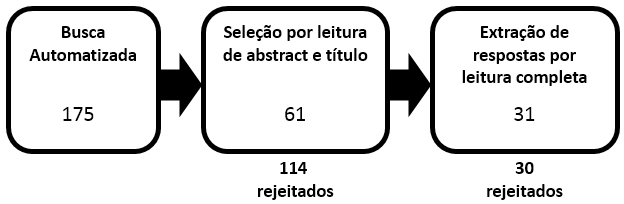
\includegraphics[scale=0.5]{images/Resumo_Metodologia}
\caption{Resumo do processo de revisão}
\label{fig:processo_revisao}
\end{figure}

\subsection{Overview dos artigos encontrados}

Destes artigos aceitos por responderem nossas questões de pesquisa, a maioria deles (68\%) foram publicados em conferências ou workshops, mas alguns (26\%) foram publicados em e o restante (6\%) como capítulos de livros da área. Veja a Tabela \ref{table:artigos_por_publicacao} para maiores detalhes.

\begin{table}[!t]
% increase table row spacing, adjust to taste
\renewcommand{\arraystretch}{1.1}
% if using array.sty, it might be a good idea to tweak the value of
% \extrarowheight as needed to properly center the text within the cells
\caption{Artigos aceitos por tipo de publicação}
\label{table:artigos_por_publicacao}
\centering
\begin{tabular}{|m{1.2cm}|m{5.5cm}|m{0.4cm}|}
\hline
Tipo & Locais de Publicação (Quantidade de artigos) & Total  \\ 
\hline\hline
Conferências ou Revistas & BWCCA(1), CIBSE(2), CICSyN(1), EmpiRE(1), ENASE(1), ICCSA(1), ICSTW(1), IEEE IREC(1), IWPSE(1), IWSM(1), JIT RE Workshop(1), MoDRE(1), RCIS(1), REFSQ(2), RSSE (1), SEAA(1), SWQD(1), XP(1), AGILE Conference(1) & 21 \\
\hline
Revistas ou Journals & IEEE Software(1), Information and Software Technology(1), International Journal of Software Engineering and Knowledge Engineering(1), Journal of Emerging Technologies in Web Intelligence(1), Journal of Object Technology(1), Journal of Software(1), Journal of Systems and Software(1), Requirements Engineering(1) & 8 \\
\hline
Livros & Engineering and Managing Software Requirements (1), Best practices guidelines for agile requirements engineering practices (1) & 2 \\
\hline
\end{tabular}
\end{table}

\begin{figure}[!t]
\captionsetup{justification=centering}
\centering
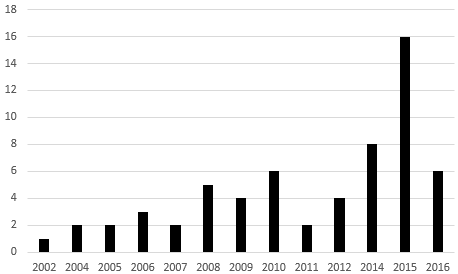
\includegraphics[scale=0.6]{images/Aceitos_ano}
\caption{Resumo dos anos de publicações aceitas}
\label{fig:aceitos_ano}
\end{figure}

\begin{figure}[!t]
\captionsetup{justification=centering}
\centering
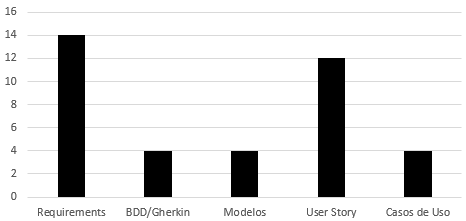
\includegraphics[scale=0.6]{images/Aceitos_formatos}
\caption{Resumo dos formatos de requisitos encontrados}
\label{fig:aceitos_formatos}
\end{figure}

\begin{figure}[!t]
\captionsetup{justification=centering}
\centering
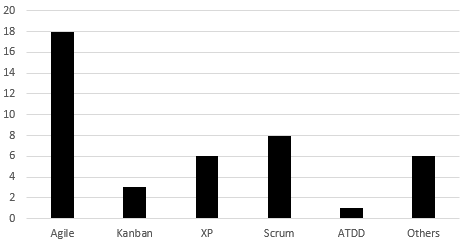
\includegraphics[scale=0.6]{images/Aceitos_metodologias}
\caption{Resumo das metodologias de desenvolvimento encontradas}
\label{fig:aceitos_metodologias}
\end{figure}

Ao se analisar a o histórico de publicações aceitas para análise, se nota como muitos artigos recentes (até 4 anos atrás) foram obtidos. Veja a Fig. \ref{fig:aceitos_ano} para maiores detalhes,

Quanto a metodologia de desenvolvimento de software e ao formato de requisito citados em cada publicação, se nota que a maioria se referia somente a requisitos e a processos ágeis de uma forma bastante genérica sem se focar em um metodologia específica ou formato específico. Ainda, dada a popularidade do método de representar requisitos descrito por \cite{Cohn_2004}, \textit{User Stories} apareceu em evidência. Vários trabalho também se focavam em mais de uma metodologia (por comparar uma com outra) ou formato de requisito (por fazer um mapeamento de um formato em outro) ao mesmo tempo, logo, múltiplas opções podem ter sido marcadas para uma mesma publicação. Para maiores detalhes, consultar a Fig \ref{fig:aceitos_formatos} e \ref{fig:aceitos_metodologias}.

\subsection{Definições de qualidade de requisitos ágeis encontradas}

A pergunta de pesquisa \textbf{QP1} procurava conhecer a definição de qualidade de requisitos em metodologias ágeis. Porém, não foi encontrado um consenso de respostas. A maioria dos artigos respondentes (51\%) não se focam em responder diretamente essa pergunta, se apoiando nos vários critérios de qualidade que cita para definir qualidade de requisitos. Já quase um terço das publicações define qualidade de requsitos como uma documentação que reflita o que o cliente deseja obter de maneira acertada, que supra as expectativas deles e transmita a equipe de desenvolvimento exatamente o que deve ser feito. Uma pequena parcela ainda trata qualidade de requisitos como um \textit{checklist} de critérios para garantir que o requisito está pronto para ser consumido pela equipe. Uma parcela igualmente pequena aponta que a ausência de problemas em requisitos garante sua qualidade. A Fig. \ref{fig:respostas_qp1} sumariza essas observações.

\begin{figure}[!h]
\captionsetup{justification=centering}
\centering
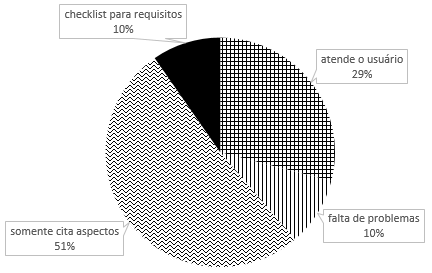
\includegraphics[scale=0.7]{images/Respostas_QP1}
\caption{Resumo das respostas sobre o conceito de qualidade de requisitos em metodologias ágeis}
\label{fig:respostas_qp1}
\end{figure}

\subsection{Aspectos de qualidade de requisitos ágeis encontradas}

Já a pergunta de pesquisa \textbf{QP2} buscava definir quas os aspectos de qualidade de requisitos eram levados em consideração em processos ágeis. Os dados da tabela \ref{table:artigos_por_aspecto} nos levam a acreditar que os aspectos tradicionais, encontrados em \cite{Babok_2015}, ainda são os mais utilizados como referência. 

Porém, técnicas alternativas como o SMART e o INVEST \cite{SMART_INVEST_2013} também foram bastante referenciadas, especialmente em critérios que não são cobertos pela escala tradicional, como a preferência por requisitos pequenos, concisos, valiosos para o cliente e com um problema bem definido a resolver. 

Ainda, a preocupação com rastreabilidade apontada em \cite{Inayat_2015} parece ser compartilhada com vários outros trabalhos, dado a quantidade de vezes que apareceu como outro critério importante.

Contudo, expressividade, uniformidade e clareza de linguagem são critérios que não aparecem com frequência. Isso evidencia que talvez a escrita e descrição do requisito não sejam a maior preocupação em metodologias ágeis, devido as práticas encontradas em \cite{Inayat_2015} que dão foco a comunicação face-a-face e requisitos iterativos, escritos gradualmente durante o ciclo de desenvolvimento. Da mesma forma, poucos artigos se preocupam com noções de valor extrínseco (quão felizes ficarão os usuários com aquela funcionalidade) \cite{KANO84} ou critérios vindo de práticas de inspeção \cite{Saito_PQM_13}.

\begin{table}[!t]
% increase table row spacing, adjust to taste
\renewcommand{\arraystretch}{1.3}
% if using array.sty, it might be a good idea to tweak the value of
% \extrarowheight as needed to properly center the text within the cells
\caption{Artigos aceitos por aspecto de qualidade de requisito}
\label{table:artigos_por_aspecto}
\centering
\begin{tabular}{|m{1.7cm}|m{5cm}|m{0.4cm}|}
\hline
Aspecto de Qua- lidade & Artigos que referenciaram & Total \\ 
\hline\hline
Completo (\cite{Babok_2015},\cite{Babok_2009}) & P8, P9, P11, P12, P13, P20, P24, P26, P33, P34, P43, P45, P47, P81, P108, P109, P114, P121, P159, P166 & 20  \\ 
\hline
Correto (\cite{Babok_2009}), preciso & P8, P9, P11, P12, P24, P26, P33, P34, P43, P45, P73, P81, P108, P109, P136, P149, P159, P160 & 18  \\ 
\hline
Testável (\cite{Babok_2015},\cite{Babok_2009},\cite{SMART_INVEST_2013}) & P2, P3, P8, P9, P11, P13, P24, P34, P40, P43, P45, P114, P121, P136, P159, P166 & 16 \\ 
\hline
Não ambíguo (\cite{Babok_2015},\cite{Babok_2009}) & P8, P9, P11, P13, P20, P24, P33, P34, P43, P47, P76, P109, P114, P121, P160, P166 & 16 \\ 
\hline
Consistente (\cite{Babok_2015},\cite{Babok_2009}), sem conflitos & P9, P11, P13, P20, P24, P33, P34, P45, P47, P48, P108, P109, P121, P136, P159, P160 & 16  \\ 
\hline
Rastreável & P9, P11, P13, P24, P40, P45, P73, P121, P136, P159 & 10 \\ 
\hline
Pequeno (\cite{SMART_INVEST_2013}), escalável, conciso & P2, P3, P9, P11, P20, P45, P114, P121, P159 & 9 \\ 
\hline
Valioso (\cite{SMART_INVEST_2013}), relevante (\cite{SMART_INVEST_2013}), orientado a um problema, orientado ao cliente & P2, P3, P9, P11, P30, P73, P114, P121, P159 & 9 \\ 
\hline
Entendível \cite{Babok_2015}, legível & P28, P34, P45, P48, P81, P109, P136, P159 & 8 \\ 
\hline
Independente (\cite{SMART_INVEST_2013}), modular & P1, P2, P3, P9, P11, P45, P114, P121, P159 & 8 \\ 
\hline
Específico (\cite{SMART_INVEST_2013}), único & P9, P11, P24, P30, P33, P109, P159 & 7 \\ 
\hline
Estimável (\cite{Babok_2015},\cite{SMART_INVEST_2013}) & P2, P3, P9, P114, P121, P136 & 6 \\ 
\hline
Negociável (\cite{SMART_INVEST_2013}) & P2, P3, P9, P114, P121 & 5 \\ 
\hline
Modificável & P33, P43, P114, P136, P159 & 5 \\ 
\hline
Viável (\cite{Babok_2015},\cite{Babok_2009}), alcançável (\cite{SMART_INVEST_2013}) & P9, P43, P109, P136, P159 & 5 \\ 
\hline
Mensurável (\cite{SMART_INVEST_2013}) & P9, P11, P20, P24, P149 & 5 \\ 
\hline
Bem formado, linguagem clara & P11, P20, P114, P121 & 4 \\ 
\hline
Criativo (\cite{KANO84}) & P3, P76 & 2 \\ 
\hline
Restrito no tempo (\cite{SMART_INVEST_2013}) & P9, P11 & 2 \\ 
\hline
Uniforme & P9, P11, P24 & 3 \\ 
\hline
Pragmático (\cite{Saito_PQM_13}) & P24 & 1 \\ 
\hline
Expressivo & P13 & 1 \\
\hline
\end{tabular}
\end{table}